%*******************************************************************************
%****************************** Fourth Chapter *********************************%*******************************************************************************
\chapter{Experiments} \label{chapter4}

% **************************** Define Graphics Path **************************
%\ifpdf
%    \graphicspath{{chapter5/figs/raster/}{chapter5/figs/PDF/}{chapter5/figs/}}
%\else
%    \graphicspath{{chapter5/figs/vector/}{chapter5/figs/}}
%\fi
%

\graphicspath{{figs/chapter4/PDF/}}


%%**************************** %Broad Purpose  *********************************
%\section*{Summary and broad purpose of the chapter}
%* How long (number of words)?


\section{Aims}
We design two experiments for human-image interaction (HII) and 
human-humanoid interaction (HHI) where participants perform simple arm 
movements repetitions.
The aims of the experiments is not only to investigate the weaknesses and 
robustness of RSS, UTDE, embedding parameters, RP and RQA metrics regarding 
different conditions presented in real-world time series data 
(noise, nonstationarity, smoothness, window size lengths and structures), 
but also to present experimental scenarios where one can observe 
how the variables that model movement variability
(e.g. complexity, predictability and activity type)
\citep{stergiou2006, vaillancourt2002, vaillancourt2003}
affect nonlinear analyses.

\section{Participants}
Twenty-three participants, from now on defined as $pN$ where $N$ is the 
number of participant, were invited for two experiments of 
simple arm movements. 
However, it is important to note that although the same number of 
participants performed the experiments, different number of participants 
were take into account for each of the experiments due to either 
technical problems with the sensors or the instructions of the experiments 
were mistakenly given.


\subsection{Human-Image Imitation Activities}
Only six participants ($p01, p04, p05, p10, p11, p15$) were considered 
for the experiment of Human-Image Imitation (HII) activities due to  
problems with the inertial sensors such as bluetooth disconnections and
drifting of time synchronisation (Section \ref{appendix:imus:issues}).
Hence, the six participants were male right-handed healthy participants 
and have a mean and standard deviation (SD) age of mean=19.5 (SD=0.83) years.


\subsection{Human-Humanoid Imitation Activities}
For the experiment of Human-Humanoid Imitation (HHI) activities, 
data for only twenty participants were analysed since the instructions 
for $p01$, who was the only left-handed, were mistakenly given in a way 
that movements were differently performed from what had been planned, 
and for participants $p13$ and $p16$ data were corrupted because of  
bluetooth communications problems with the sensors 
(Section \ref{appendix:imus:issues}).
With that in mind, all of the 20 participants were right-handed 
healthy participants, being four females and sixteen males, with 
a mean and standard deviation (SD) age of mean=19.8 (SD=1.39) years.





\section{Equipment}
During the experiments, time series were collected with four neMEMSi 
Inertial Measurement Units (IMUs) using a sampling rate of 50Hz 
\citep{Comotti2014}. neMEMSi sensors provide tri-axial time series from 
the accelerometer, gyroscope and magnetometer sensors and quaternions.
See Appendix \ref{appendix:imus} for further technical information of 
 NeMEMSi IMU sensors.

With regard to the human-humanoid imitation activities, NAO, 
a humanoid robot from Aldebaran \citep{gouaillier2009}, 
were programmed with choreographer to perform horizontal and vertical 
arm movements.
See Appendix \ref{appendix:nao} for further technical information 
regarding NAO and the code of NAO's
movements. 



\section{Ethics}
The experiments of this thesis were conducted in November 2016 and
participants confirmed reading and understanding the participant information 
sheet of the experiments and were able to withdraw from the experiment 
at any time without giving any reason.
The design of the experiments is adhered to University of Birmingham 
regulations, data were anonymised and videos were stored 
only a personal computer in accordance with the Data Protection Act 1998.
Refer to Appendix \ref{appendix:c} for further information about the 
ethics, online participation information sheets and experiment check list.


\section{Experiments}

\subsection{Human-Image Imitation Activities} \label{sec:experiment:hii}
In the experiment of human-image imitation (HHI), four wearable IMUs sensors 
were used and attached to the right hand of the participant 
(Figure~\ref{fig:hii} A,D). 
Then, participants performed two experiments: 
(i) an unconstrained arm movement imitation activity where participants 
only receive instructions and look at images of the arm movements, and
(ii) a constrained experiment where participants hear a beat 
to synchronise their arm movements. 

\subsubsection{Arm movements following an image while not hearing a beat}
Participants received instructions to perform unconstrained upper arm 
movements while only looking an image for
\begin{itemize}[noitemsep,topsep=0pt]
\item ten repetitions of horizontal arm movement at their comfortable velocity
(Fig. \ref{fig:hii}(A, B, C)), 
\item ten repetitions of vertical arm movement at their comfortable velocity 
(Fig. \ref{fig:hii}(D, F, E)),
\item ten repetitions of horizontal arm movement at a faster velocity than 
the comfortable velocity but not at their fastest velocity 
(Fig. \ref{fig:hii}(A, B, C)), and 
\item ten repetitions of vertical arm movement at a faster velocity than the 
comfortable velocity but not at their fastest velocity
(Fig. \ref{fig:hii}(D, F, E)).
\end{itemize}

\subsubsection{Arm movements following an image while hearing a beat}
Participants received instructions to perform constrain upper arm movements 
while listening a beat to constraint their movements. 
\begin{itemize}[noitemsep,topsep=0pt]
\item ten repetitions of horizontal arm movement at normal velocity
(Fig. \ref{fig:hii}(A, B, C)), 
\item ten repetitions of vertical arm movement at normal velocity
(Fig. \ref{fig:hii}(D, F, E)), 
\item ten repetitions of horizontal arm movement at faster velocity and
(Fig. \ref{fig:hii}(A, B, C)), and 
\item ten repetitions of vertical arm movement at faster velocity
(Fig. \ref{fig:hii}(D, F, E)).
\end{itemize}

To visualise the time series of the previous activities, Figs 
\ref{fig:hii-sts} show time series using smoothed gyroscope of Y and Z 
for the sensor HS01 of participant 01.
%%---------------------------------(FIGURE)-------------------------------------
\begin{figure}
  \centering
  \includegraphics[width=1.0\textwidth]{hii}
    \caption{
	{\bf Human-image imitation (HII) activities.} 
		%Human-image imitation (HHI) activities for 
		(A) HII of horizontal arm movement, 
		(B) image of the profile view for horizontal arm movement,
		(C) image of the top view for horizontal arm movement,
		(D) HII of vertical arm movement, 
		(E) image of the profile view for vertical arm movement, and
		(F) image of the top view for horizontal arm movement.
		(B, C, F and E) show '(((BEAT)))' to indicate the participants
		arm movements synchronisation when hearing a beat.
        }
    \label{fig:hii}
\end{figure}
%%---------------------------------(FIGURE)------------------------------------
%%---------------------------------(FIGURE)-------------------------------------
\begin{figure}[!h] 
  \centering
  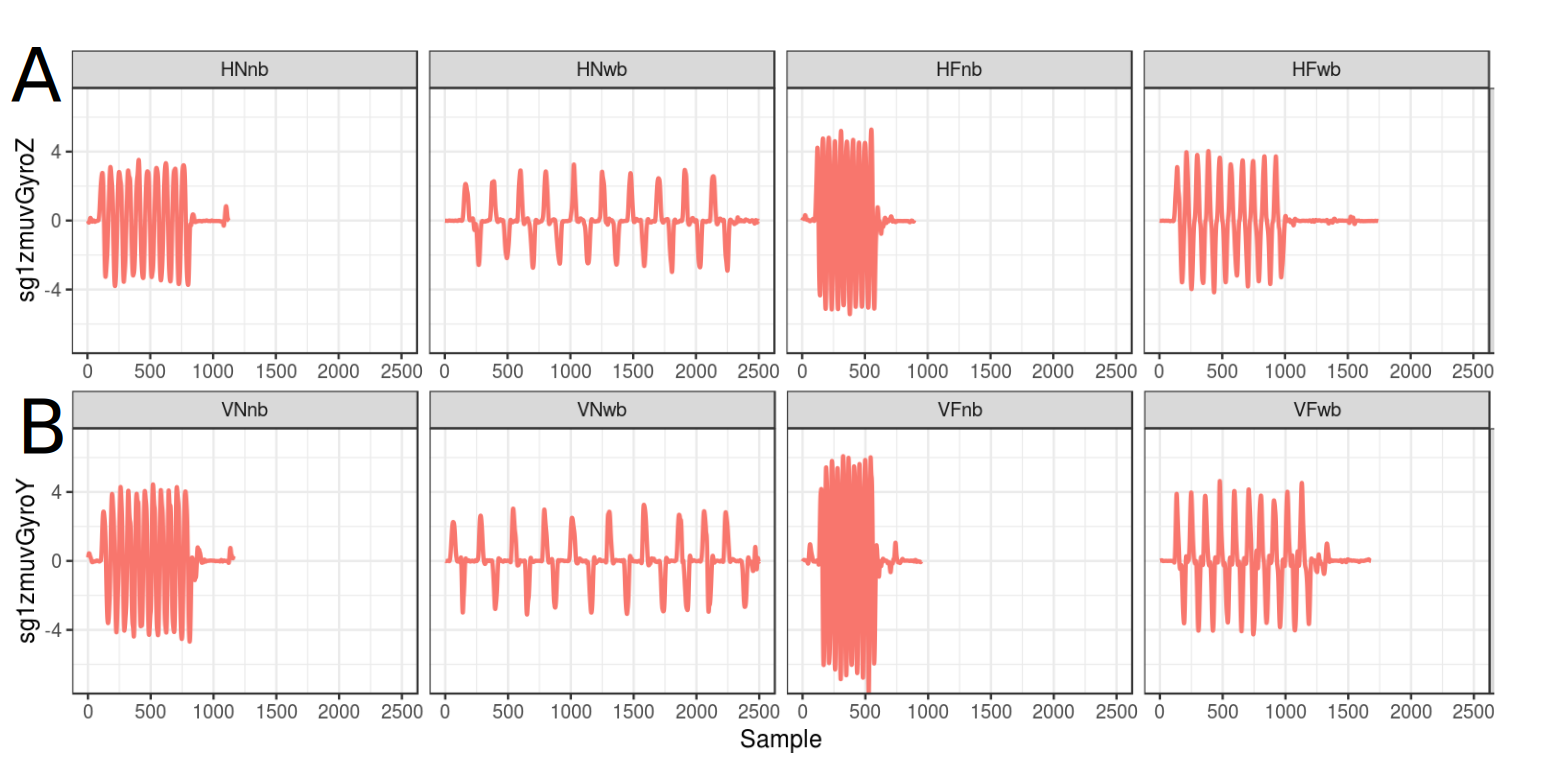
\includegraphics[width=1.0\textwidth]{hii-sts}
    \caption{
	{\bf Time series for horizontal and vertical arm movements.} 
		Time series of smoothed data from gyroscope sensor 
		(sg1zmuvGyroZ and sg1zmuvGyroY) of participant 01 
		with sensor HS01 for different velocity arm movements: 
		(A) Horizontal Normal with no beat (HNnb),
			Horizontal Normal with beat (HNwb), 
			Horizontal Faster with no beat (HFnb) and
			Horizontal Faster with beat (HFwb), and 
		(B) Vertical Normal with no beat (HNnb),
			Vertical Normal with beat (HNwb), 
			Vertical Faster with no beat (HFnb) and
			Vertical Faster with beat (HFwb).
		R code to reproduce the figure is available \cite{hwum2018}.
        }
	\label{fig:hii-sts}
\end{figure}
%%---------------------------------(FIGURE)------------------------------------






\subsection{Human-Humanoid Imitation Activities} \label{sec:experiment:hhi}
For the human-humanoid imitation (HHI) experiment four wearable IMUs sensors 
were used in which two sensors were attached to the right hand of 
the participant and two sensors were attached to the left hand of 
the humanoid robot (Figure~\ref{fig:hri} A,C).
Then, in the face-to-face imitation activity, each participant was asked 
to imitate repetitions of simple horizontal and vertical arm movements 
performed by the humanoid robot in the following conditions:
\begin{itemize}[noitemsep,topsep=0pt]
\item ten repetitions of horizontal arm movement at normal (HN) and faster (HF) 
velocity (Fi.~\ref{fig:hri} A), and
\item ten repetitions of vertical arm movement at normal (VN) and faster (VF) 
velocity (Fig.~\ref{fig:hri} C).
\end{itemize}
%%---------------------------------(FIGURE)-------------------------------------
\begin{figure}
  \centering
  \includegraphics[width=1.0\textwidth]{hri}
    \caption{
	{\bf Human-humanoid imitation activities.} 
		Face-to-face human-humanoid imitation (HHI) activities for 
		(A) HHI of horizontal arm movement, 
		(B) Humanoid horizontal arm movement,
		(C) HHI of vertical arm movement, and 
		(D) Humanoid vertical arm movement.
        }
    \label{fig:hri}
\end{figure}
%%---------------------------------(FIGURE)------------------------------------
The normal and faster velocity of arm movements is defined by the duration in 
number of samples of one repetition of NAO's arm movements.
We select NAO's arm movements duration to distinguish between normal and 
faster arm movements as the movements from the humanoid robot have less 
variation between repetition to repetition. 
The duration for one repetition of the horizontal 
arm movement at normal velocity, HN, is about 5 seconds considering that 
each repetition last around 250 samples. For horizontal arm movement at 
faster velocity, HF, each repetition were performed in around 2 seconds 
which correspond to 90 samples of data. 
The vertical arm movement at normal velocity, VN, were performed  in 6 seconds 
which is around 300 samples of data.
For vertical arm movement at faster velocity, VF, each repetition lasts 
about 2.4 seconds which correspond to 120 samples of data.
To visualise the distinction between normal and faster velocity for horizontal 
and vertical arm movements, Fig~\ref{fig:sts} shows smoothed time series 
for axes Z and Y of the gyroscope sensors with four window lengths: 
2-sec (100-samples), 5-sec (250-samples), 10-sec (500-samples) 
and 15-sec (750-samples).
%%---------------------------------(FIGURE)-------------------------------------
\begin{figure}[!h] 
  \centering
  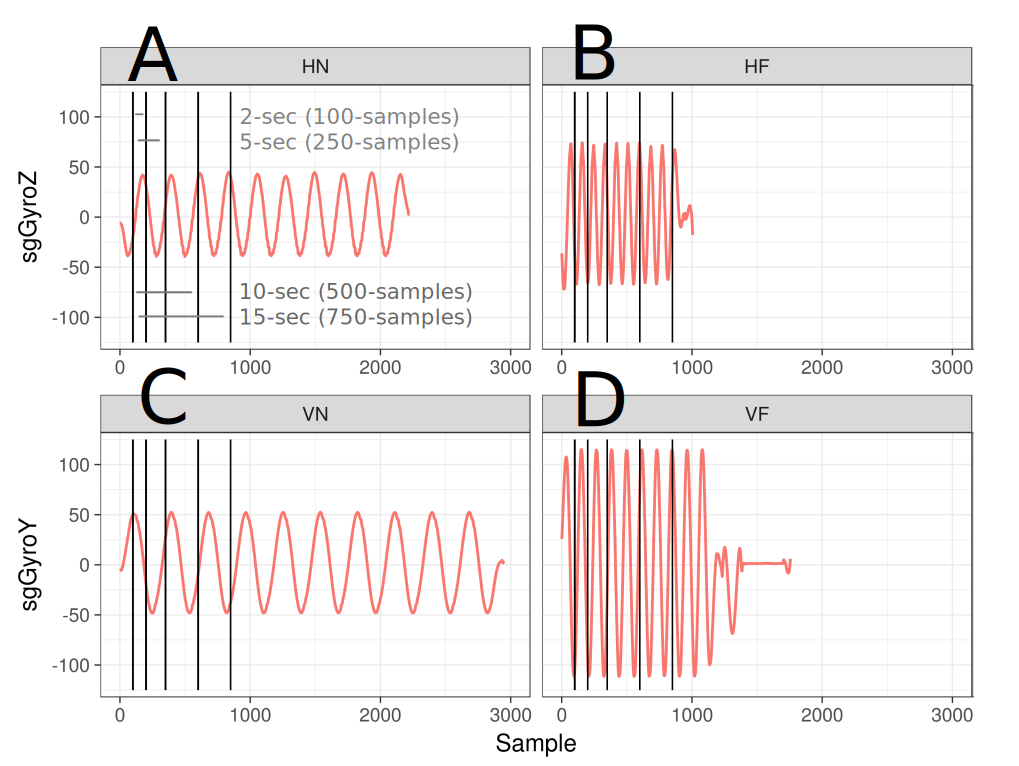
\includegraphics[width=1.0\textwidth]{sts}
    \caption{
	{\bf Time series duration of horizontal and vertical arm movements.} 
		Time series of smoothed data from gyroscope sensor 
		for different velocity arm movements performed by NAO: 
		(A) Horizontal Normal arm movement, HN, 
		(B) Horizontal Faster arm movement, HF,
		(C) Vertical Normal arm movement, VN, and 
		(D) Vertical Faster arm movement, VF.
		Additionally, (A) shows window sizes for 2-seconds 
		(100 samples), 5-seconds (250 samples), 
		10-seconds (500 samples) and 15-seconds (750 samples)
		which are also presented in (B), (C) and (D).
		R code to reproduce the figure is available \cite{hwum2018}.
        }
	\label{fig:sts}
\end{figure}
%%---------------------------------(FIGURE)------------------------------------

\section{Processing of time series} \label{sec:preparation_timeseries}

\subsection{Raw time-series}
Considering the work of \cite{shoaib2016} which provided evidence 
of an improvement in recognition activities when combining data 
from accelerometer and gyroscope, analysis for time series, in this thesis, 
uses only the accelerometer and gyroscope of the IMU sensors which leaves 
magnetometer and quaternions for future investigations because of 
their possible variations with regard to magnetic disturbances.

Time series from the accelerometer are defined by triaxial time series 
$A_x(n)$, $A_y(n)$, $A_z(n)$ which forms the matrix $\boldsymbol{A}$ 
(Eq.~\ref{eq:A}), and the same for data from the gyroscope which is 
defined by triaxial time-series of $G_x(n)$, $G_y(n)$, $G_z(n)$ representing 
the matrix $\boldsymbol{G}$ (Eq.~\ref{eq:G}). Both triaxial time series of 
each sensor, $a$ and $g$, are denoted with its respective axes 
subscripts $x,y,z$, where $n$ is the sample index  and $N$ is the same 
maximum length of all axes for the time series.
Matrices  $\boldsymbol{A}$ and $\boldsymbol{G}$ are represented as follow
%%---------------------------------(EQUATION)-----------------------------------
\begin{equation}\label{eq:A}
\boldsymbol{A} =
\begin{pmatrix}
  A_x(n) \\
  A_y(n) \\
  A_z(n)
\end{pmatrix}
=
\begin{pmatrix}
 a_x(1),a_x(2),\dots,a_x(N) \\
 a_y(1),a_y(2),\dots,a_y(N) \\
 a_z(1),a_z(2),\dots,a_z(N) 
\end{pmatrix},
\end{equation}
%%---------------------------------(EQUATION)-----------------------------------
%%---------------------------------(EQUATION)-----------------------------------
\begin{equation}\label{eq:G}
\boldsymbol{G} =
\begin{pmatrix}
 G_x(n) \\
 G_y(n) \\
 G_z(n)
\end{pmatrix}
=
\begin{pmatrix}
 g_x(1),g_x(2),\dots,g_x(N) \\
 g_y(1),g_y(2),\dots,g_y(N) \\
 g_z(1),g_z(2),\dots,g_z(N) 
\end{pmatrix},
\end{equation}
%%---------------------------------(EQUATION)-----------------------------------
where $n$ is the sample index  and $N$ is the same maximum length of all axes 
for the time series.


\subsection{Postprocessing time-series}
After the collection of raw time-series from four NeMEMsi sensors,
time synchronisation alignment and interpolation were performed 
in order to create time series with the same length and synchronised time.
We refer the reader to Appendix~\ref{appendix:b} for technical information 
about the time synchronisation process and IMU sensors.

\subsection{Normalization of time-series}
Tim series are normalised to have zero mean and unit variance 
using sample mean and sample standard deviation \citep{loffe2015}.
The sample mean and sample standard deviation using $x(n)$ is given by
%%---------------------------------(EQUATION)-----------------------------------
\begin{equation}\label{eq:ms}
\mu_{x(n)}= \frac{1}{N} ( \sum_{i=1}^N x(i) ), \quad  \sigma_{x(n)} =  \sqrt{ \frac{  \sum_{1=1}^N ( x(i) - \mu_{x(n)} )^2 }{ N-1 }  },      
\end{equation}
%%---------------------------------(EQUATION)-----------------------------------
then the normalised data, $\hat{x}(n)$, is computed as follows
%%---------------------------------(EQUATION)-----------------------------------
\begin{equation}\label{eq:normalization}
\hat{x} (n) = \frac{   x(n) -  \mu_{x(n)}  }{   \sigma_{x(n)} }.   
\end{equation}
%%---------------------------------(EQUATION)-----------------------------------

\subsection{Smoothing time-series}
Using a low-pass filter is the common way to either capture the low 
frequencies (below 15 Hz) that represent \%99 of the human body 
energy or to get the gravitational and body motion components of 
accelerations (below 0.3 Hz) \citep{anguita2013}.
However, for this thesis the main focus is on the conservation of the 
structure of the time series in terms of the width and heights where, 
for instance, a Savitzky-Golay filter can help to accomplish such task 
\citep{press1992}. Savitzky-Golay filter is based on the principle of moving 
window average which preserves the area under the curve (the zeroth moment)
and its mean position in time (the first moment) but the line width 
(the second moment) is violated and that results, for example, in the case 
of spectrometric data where a narrow spectral line is presented with 
reduced height and width. 
The aim of Savitzky-Golay filtering is hence to find the filter coefficients 
$c_n$ that preserve higher momentums which are based on local least-square 
polynomial approximations 
\citep{savitzkygolay1964, press1992, schafer2011}.
Therefore, Savitzky-Golay coefficients are computed using an R function 
\texttt{sgolay(p,n,m)} where \texttt{p} is the filter order, 
\texttt{n} is the filter length (must be odd) 
and \texttt{m} is the $m$-th derivative of the filter coefficients 
\citep{Rsignal}. Smoothed signal is represented with a tilde over the 
original signal: $\tilde{x}(n)$.



\subsection{Window size of time-series}
With regard to the window size, \cite{shoaib2016} compared 
seven window lengths (2, 5, 10, 15, 20, 25, 30 seconds)
and combination of inertial sensors (accelerometer, gyroscope and linear 
acceleration sensor) in activity recognition performance for repetitive 
activities (walking, jogging and biking) and less repetitive activities 
(smoking, eating, giving a talk or drinking a coffee).
Similarly, \cite{shoaib2016} experimented with different window size effect 
to conclude that the increase of window size improved the recognition of 
complex activities because these required a large window to learn the 
repetitive motion patterns. Also, \cite{shoaib2016} concluded that the use 
of large window size improve the recognition performance of less repetitive 
activities which mainly involve random hand gestures.

For the activities in this thesis which are mainly repetitive, we selected 
only four window sizes: 2-s window (100 samples), 5-s window (250 samples), 
10-s (500 samples) and 15-s window (750 samples) (Figure~\ref{fig:sts}).




